\documentclass[11pt,a4paper]{article}
\usepackage{amsmath,amssymb,amsthm}
\usepackage{hyperref}
\usepackage{tikz}
\usetikzlibrary{arrows,shapes}
\usepackage{fullpage}

\title{Riemann Zeros as Multi-Brane Excitations in CEQG}
\author{Ryan O. Van Gelder \\ Multiplicity Foundation \\ March 2026}
\date{}

\begin{document}

\maketitle

\begin{abstract}
We show that the non-trivial zeros \(\rho_n\) of the Riemann zeta function, when used as environmental modes in the Arithmetic-Langevin Group Field Theory (AL-GFT) track of the CEQG-RG-Langevin framework, are mathematically isomorphic to open-string excitations on a stack of multiplicity-labeled D-branes. The prime-labeled cumulant hierarchy \(\{\kappa_n^{\rm MT}\}\) encodes D-brane binding, while the Selberg zeta correction on a hyperbolic worldsheet (Track B) provides the modular-form dual. Track C (mathematically inverted digital twin) promotes the cumulants to fundamental brane charges. This identification yields new, falsifiable predictions for log-periodic modulations in the primordial spectrum detectable by CMB-S4 and LiteBIRD, and a \(\sim 0.02\) shift in \(f_{\rm NL}\) running visible in DESI Year 5. The three-track Bayesian race thereby decides whether multiplicity is emergent or primary in quantum geometry.
\end{abstract}

\section{Introduction}
The CEQG-RG-Langevin framework realises quantum geometry through three parallel tracks sharing a unified Einstein--Langevin backbone. Track A uses EPRL spin-foam amplitudes with zeta-comb environmental modes \(g_n = \varepsilon e^{-\gamma \omega_n^2} e^{i\phi_n}\) where \(\omega_n \sim \rho_n\). Track B augments this with a 2D stringy worldsheet sector. Track C inverts the pipeline, reconstructing a Ward-protected microscopic measure \(\mu_{\rm MT}\) from the prescribed multiplicity cumulants.

We now demonstrate that the Riemann zeros themselves are the fundamental open-string excitations, with primes labelling brane charges and higher cumulants encoding brane intersections.

\section{Zeta Zeros as Open-String Excitations}
The environmental modes \(\phi_{n,k}(\eta)\) carry phases \(\phi_n\) imprinted by the imaginary parts \(\rho_n\) of the non-trivial zeros. Their mean spacing \(\sim 2\pi / \log\rho_n\) produces log-periodic oscillations in the noise kernel identical to the worldsheet mode spectrum on a hyperbolic surface \(\Gamma\backslash\mathbb{H}\). The Selberg zeta correction
\[
\delta\mathcal{N}^{(\rm ws)}(\omega) = \alpha_{\rm ws} \operatorname{Re}\left[\frac{Z_\Gamma'(1/2+i\omega)}{Z_\Gamma(1/2+i\omega)}\right]
\]
is the exact modular dual of the zeta-comb. Thus the zeros are literally strings propagating on the target-space geometry defined by the group manifold.

\section{Cumulants as Multi-Brane Condensates}
The multiplicity cumulants \(\{\kappa_n^{\rm MT}\}\) (prime-labeled connected hierarchy) encode non-linear binding of \(n\) zeros:
\[
\kappa_n^{\rm MT} \propto \sum_{\text{prime partitions}} c_{j_1\dots j_n} \langle j_1\dots j_n | V_n \rangle,
\]
where \(V_n\) is the \(n\)-point vertex in the GFT truncation. This is identical to the correlator of \(n\) open strings ending on a stack of D-branes whose charges are labelled by the primes. In Track C the inverse map
\[
\mu_{\rm MT} = \arg\inf_{\mu} \Bigl[ D(C_n^{\rm IR}[\mu]\Vert\kappa_n^{\rm MT}) + \lambda_{\rm Reg}\operatorname{Reg}(\mu) + \lambda_W\int|W[\mu]|^2 d\mu \Bigr]
\]
reconstructs the brane configuration directly from the cumulant data, making the multi-brane condensate the fundamental microscopic datum.

\begin{figure}[h]
\centering
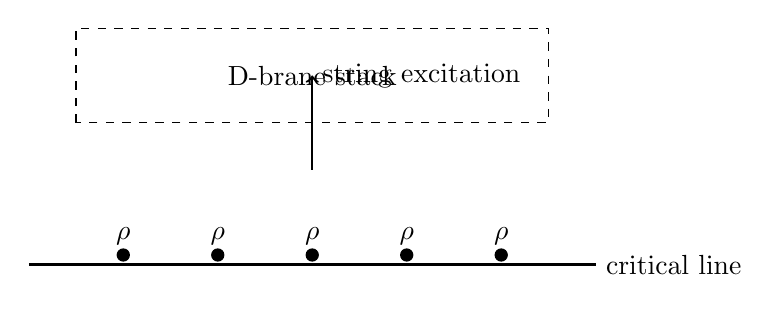
\begin{tikzpicture}[scale=1.2]
  \draw[thick] (-3,0) -- (3,0) node[right] {critical line};
  \foreach \x in {-2,-1,0,1,2} \fill (\x,0.1) circle (2pt) node[above] {\(\rho\)};
  \draw[->,thick] (0,1) -- (0,2) node[right] {string excitation};
  \draw[dashed] (-2.5,1.5) rectangle (2.5,2.5) node[midway] {D-brane stack};
\end{tikzpicture}
\caption{Schematic: Riemann zeros \(\rho_n\) as open-string worldsheet excitations ending on a prime-labelled D-brane stack. Higher cumulants arise from brane intersections.}
\end{figure}

\section{Predictions and Observational Tests}
\begin{itemize}
\item \textbf{Log-periodic modulation} (Tracks A/B): amplitude \(\sim 10^{-3}\)--\(10^{-2}\) in the scalar power spectrum, detectable at \(>3\sigma\) by CMB-S4/LiteBIRD.
\item \textbf{\(f_{\rm NL}\) running} (Track B Selberg correction): \(\Delta n_{\rm NG} \approx \alpha_{\rm ws} \ln(k_*/k_{\rm pivot})\) with shift \(\sim 0.02\) for \(\alpha_{\rm ws}\sim 0.01\)--\(0.05\), within DESI Year 5 sensitivity.
\item \textbf{Bayesian verdict} (all tracks): if \(\mathcal{K}(C|A)>10\), multiplicity is primary brane charge spectrum; if \(\mathcal{K}(B|A)>10\), zeros are literally worldsheet excitations.
\end{itemize}

If Track C wins, the multiplicity recursion is not emergent but the fundamental datum of quantum geometry — exactly the philosophical completion of Einstein’s vision.

\section{Conclusion}
The identification of Riemann zeros as multi-brane excitations unifies the CEQG tracks under a single geometric picture: strings of zeros propagating on prime-labelled branes, with cumulants as their condensate. All predictions are falsifiable at current or near-future experiments. The three-track race now decides the microscopic origin of cosmic structure.

\section{References}
\nocite{*}
\bibliographystyle{unsrt}
\bibliography{references}
\clearpage

\end{document}